\section{Methods - Convection Schemes}
\subsection{Testing Methodology}
First a simple convection scheme will be tested. This scheme will implement none of the optimization methods discussed in this report and represents the full N-Body problem. This scheme is implemented and tested so the optimizations can be compared to to a result where no optimizations are present. Schemes will be assessed based on two parameters, their performance (computational cost) and accuracy
\\\\
The performance of the schemes will be assessed by finding the time taken to calculate a set number of increments with a range of element counts. Hence all variables are kept constant except element count, and the effect of this on computational cost is measured. From this data the performance of the schemes can be compared against the optimized case. However by taking data over a range of element counts, the trend of how computational cost increases with element count can be found. The use of this is twofold. Firstly a smooth consist trend is expected, so noise or errors present in the data can be assessed. Secondly the theoretical trends presented in the theory section can be assessed for accuracy (I.E the biasing scheme should reduce to a $ON$ problem).
\\\\
As the schemes run through a set range of iterations error will compound on the position of each element as a result of approximations made by the schemes. This will lead to a discrepancy between the positions calculated by a given scheme and the unoptimized case. The distance between these two positions is represented by the vector $\vec{D}$. To quantify the positional error, the magnitude of the vector from the unoptimized case to the optimized case if found, this is done via Pythagoras shown in equation \ref{eq:pythag} where subscripts N and S represent the position given by the scheme in question and the simple unoptimized case respectively.

\begin{equation}
\label{eq:pythag}
|\vec{D}|=\sqrt{(x_N-x_s)^2+(y_N-y_S)^2+(z_N-z_S)^2}
\end{equation}

As shown in equation \ref{eq:NonDimension1}, once the vector $\vec{D}$ is found it is divided by the magnitude of the vector from the initial point of a given element to its ending position during the simulation, this is denoted as the vector $\vec{M}$

\begin{equation}
\label{eq:NonDimension1}
\vec{E_{Element}}=\frac{\vec{D}}{\vec{M}}
\end{equation}

This results in a measure where a value of 0 represents no impact on accuracy and a value of 1 the worst case, the elements still inhabit their starting positions. This is still a measure for a single element, to quantify the error for a given situation the sum of this measure for all elements is found. This sum is then divided by the amount of elements, this is done so that a value of 1 still maintains its meaning of reative to the element starting positions, this is shown in equation \ref{eq:NonDimension2}
\begin{equation}
\label{eq:NonDimension2}
\vec{E}=\frac{1}{N}\sum{\vec{E_{Element}}}
\end{equation}

Total accumulated error (error norms) was not selected as with increased element count the error may be seen to increase due to the increased fidelity even when the positional  error on a given element decreases.
\\\\
The initial conditions influences how the elements move during the iterations, hence selection of initial conditions is not arbitrary and should yield non-trivial results. The initial conditions chosen for this simulation were designed to emulate the shape of the wake the simulation is being developed for. This consisted of a planar grid with vorticity seeded at two parallel edges of the grid. 
\\\\
This poses two advantages. Firstly the situation is close to the situation that is to be simulated. Secondly, it provides an ideal way to increase element count linearly. This is done by extending the planar grid in a single dimensions. For example going from a 10x10 grid to a 10x11 grid. 
\\\\
Each convective scheme has separate parameters that can be tuned to achieve a different balance of accuracy and performance, these are discussed in their respective sections.

\subsubsection{Simple Convection - Unity Implementation}
The simple convection code represents the unoptimized N-Body problem. It is the simplest implementation and provides a benchmark for the other schemes to be compared against.
\\\\
The convective section of the vortex method is shown in listing \ref{list:SimpleConvection}, this section of code is responsible for implementing the Biot-Savart law. Elements are created in a planar grid shape, any element can be specified by its position on this grid. The position and vorticity of elements are stored in the 2d arrays $elementPositions[x,y]$ and $elementVorticity[x,y]$ respectively, the index of these arrays refer to the position of the given element on the initial grid.
\\\\
The code works by cycling through the entire grid, this is done via the two for loops on lines 2 and 4. This procedure allows for every element to be selected. Once every element is selected, every other element must be selected, hence the grid must be cycled through again, this is performed by the for loops on lines 10 and 12. This results in a procedure that cycles through all element, for every element, hence it is necessary to check that for a given element, the routine has not selected itself for consideration. This is done via the evaluation on line 16.
\\\\
Before the Biot-Savart law can be implemented the radius between the elements needs to be calculated, this is done on line 20. The Biot-Savart law is then implemented on line 21.

\begin{listing}[H]
\begin{minted}[linenos,breaklines]{csharp}
//for loop to cycle through all elements
        for (int xN = 0; xN < xSize; xN++)
        {
            for (int yN = 0; yN < ySize; yN++)
            {
                //Reset the velocity field
                elementVelocity[xN, yN] = Vector3.zero;

                //Now that every element is going to be cycled through, the elements need to be cycled through again
                for (int xC = 0; xC < xSize; xC++)
                {
                    for (int yC = 0; yC < ySize; yC++)
                    {

                        //Check an element cannot convect with itself
                        if (xN != xC && yN != yC)
                        {

                                //Calcuate Influence
                                Vector3 r = elementPosition[xN, yN] - elementPosition[xC, yC];
                                elementVelocity[xN, yN] += (1f / (4f * Mathf.PI)) * (Vector3.Cross(elementVorticity[xC, yC], r) / (Mathf.Pow(r.magnitude, 2)));
                            
                        }
                    }
                }

            }
        }
\end{minted}
\caption{Unoptimized Convection Scheme Implemented in C\#}
\label{list:SimpleConvection}
\end{listing}

\subsubsection{Biasing - Tuning Parameters}
Both distance based and vorticity based biasing schemes are to be tested. Firstly the computational time for a range of element counts will be found for the same range as the simple unoptimized case so that the data may be compared. The data is used
\\\\
To asses the associated increase of decrease in overhead from the schemes the computational time for the maximum grid size will be recorded for a range of biasing factors. The range of biasing factors are determined by taking 120\% of the maximum value (maximum radius between two elements, or magnitude of vorticity of the convecting element). A range is specified with biasing factors more than the maximum value so that in the last section of the range the biasing value  is not used. By doing this the increased overhead accountable solely due to the evaluation process can be quantified.

\subsubsection{Biasing - Unity Implementation}
To implement a biasing scheme the convective scheme presented in listing \ref{list:SimpleConvection} was modified to include an additional evaluation before the Biot-Savart law is implemented. Both distance based and vorticity based biasing was implemented.
\\\\
The distance based biasing implementation is shown in listing \ref{list:DistanceBias}. The radius is calculated on line 2, this is used for the evaluation made on line 5

\begin{listing}[H]
\begin{minted}[linenos,breaklines]{csharp}
//Calcuate Influence
 Vector3 r = elementPosition[xN, yN] - elementPosition[xC, yC];

//Check if the radius is small enough to be considered
 if (r.magnitude < radiusBias)
 {
    elementVelocity[xN, yN] += (1f / (4f * Mathf.PI)) * (Vector3.Cross(elementVorticities[xC, yC], r) / (Mathf.Pow(r.magnitude, 2)));
 }
\end{minted}
\caption{Distance based biasing system implemented in C\#}
\label{list:DistanceBias}
\end{listing}

The implementation of a vorticity based biasing system is shown in listing \ref{list:VorticityBias}. The evaluation is made on line 2. The implementation differs here is that the evaluation procedure relies upon a variable, $elementVorticity.magnitude$, that is not required for the implementation of the Biot-Savart law. Conversely the distance based biasing scheme used the radius between the two elements which was used in the implementation of the Biot-Savart law. Hence it is expected that the vorticity based biasing system represents a larger overhead than the distance based biasing system.

\begin{listing}[H]
\begin{minted}[linenos,breaklines]{csharp}
//Bias based on vorticity
if (elementVorticity[xC,yC].magnitude < radiusBias)
{

	//Calculate Radius
	Vector3 r = elementPosition[xN, yN] - elementPosition[xC, yC];
                                
	//Implement Biot-Savart Law
	elementVelocity[xN, yN] += (1f / (4f * Mathf.PI)) * (Vector3.Cross(elementVorticies[xC, yC], r) / (Mathf.Pow(r.magnitude, 2)));

}
\end{minted}
\caption{Vorticity based biasing system implemented in C\#}
\label{list:VorticityBias}
\end{listing}

\subsection{Predictive Clustering - Fixed Cluster Size - Tuning Parameters}
The fixed scale clustering system will be tested for a range of cluster sizes. The initial conditions and number of iterations tested are the same as for the simple convection case, this allows for compariosn of performance and accuracy against the data sets. Computational time and accuracy will be assessed against the simple case. Three cluster sizes will be tested, $1x1$, $3x3$ and $5x5$.
\\\\
A cluster size of $1x1$ was selected as this refers to a situation where no clustering is taking place, however the infrastructure is still in place to handle the clustering system. So the increase in time taken over the unoptimized case is accountable to this additional infrastructure. Hence the discrepancy in these times can be used as a measure of how cumbersome the infrastructure is.
\\\\
The sizes $3x3$ and $5x5$ were selected as they were the only sizes that gave a suitable resolution of data points over the range tested. The grid sizing used must be a multiple of the cluster size. For example, for a $5x5$ cluster 5 different grid sizes were used, $15x5$, $15x10$... to $15x25$. However for a $3x3$ cluster there are 7 possible grid sizes in the range.
\\\\
As the grid size must be a multiple of the cluster size  the accuracies cannot be assessed at a grid size of $15x20$ like the biasing scheme were assessed as the the $3x3$ cluster size cannot be used for this grid size. Instead the accuracies will be assessed at a grid sizing of $15x15$. Hence the values of error found for the biasing schemes are not perfectly comparable to those for this data set. However, as number of iterations are constant (which represents the major increase in error through the summation of truncation errors) and the influence of an element decreases with distance (which is increased with a larger grid) these error values should still be a good indicator.
\\\\
\subsubsection{Fixed Cluster Size - Unity Implementation}
Listing \ref{list:FixedCluster} shows a fixed size cluster scheme implemented in Unity. The code has been compacted in order to be shown here (though no lines have been appended), the full version is included in the appendix. Elements are specified in the same way as the simple convection scheme, by their initial grid position. This scheme implements square clusters based upon their grid position. The function was defined to be applicable to any situation, hence the cluster size or grid dimensions are not explicitly defined in the script, instead they can be defined and changed in the program with no need for the script to be modified.
\\\\
The script works by first cycling through the clusters, this is done via the for loops on lines 2 and 4. This results in a procedure where all clusters are cycled through, the individual elements in every cluster need to be cycled through. This is achieved via an additional two for loops on lines 7 and 9. This results in a procedure where all elements are cycled through.
\\\\
Now all elements are cycled through they must be convected by either elements or clusters. Elements and clusters are handled separately. The current element is convected with every other element in its cluster, this is done between lines 14 and 27. This section of code is identical to the the simple convection script, however it is applied for only the elements in current cluster. The current element is then convected by every cluster except its own, this is done between lines 30 and 40. This code again is very similar to the simple convection script, however the only difference being $clusterPosition$ and $clusterVorticity$ are used instead of $elementPosition$ and $elementVorticity$.

\begin{listing}[H]
\begin{minted}[linenos,breaklines]{csharp}
//First Cycle through all clusters
for (int xC = 0; xC < (xSize/clusterSize); xC++)
{
for (int yC = 0; yC < (ySize/clusterSize); yC++)
{
//Now we need to consider every element in the clsuter
for (int xI = 0; xI < clusterSize; xI++)
{
for (int yI = 0; yI < clusterSize; yI++)
{
//We need to reset their velocities so they dont add up
elementVelocity[(xC * clusterSize) + xI, (yC * clusterSize) + yI] = Vector3.zero;
//Now we need to cycle through the individual elements in that cluster
for (int xIC = 0; xIC < clusterSize; xIC++)
{
for (int yIC = 0; yIC < clusterSize; yIC++)
{                     
//Now we need to check that we're not convecting the element with itself
if (xI != xIC && yI != yIC)
{
//now we need to find the radius
Vector3 Radius = elementPosition[(xC * clusterSize) + xI, (yC * clusterSize) + yI] - elementPosition[(xC * clusterSize) + xIC, (yC * clusterSize) + yIC];
//Now we can implement the biot-savart law
elementVelocity[(xC * clusterSize) + xI, (yC * clusterSize) + yI] += (1.0f / (4.0f * Mathf.PI)) * (Vector3.Cross(vorT[(xC * clusterSize) + xIC, (yC * clusterSize) + yIC], Radius) / Mathf.Pow(Radius.magnitude, 2));
}
}
}
//Now we need to convect the given element with the clusters
//First we cycle through all the clusters
for (int xCC = 0; xCC < (xSize/clusterSize); xCC++)
{for (int yCC = 0; yCC < (ySize/gridSpacing); yCC++)
{
//Now we need to check that we're not going to convect with the clsuter the element is inside of
if (xC != xCC && yC != yCC){
//Now we need to calculate the radius
Vector3 Radius = elementPosition[(xC * clusterSize) + xI, (yC * clusterSize) + yI] - clusterPosition[xCC, yCC];//Now we can implement the biot-savart law
elementVelocity[(xC * clusterSize) + xI, (yC * clusterSize) + yI] += (1.0f / (4.0f * Mathf.PI)) * (Vector3.Cross(clusterVorticity[xCC, yCC], Radius) / Mathf.Pow(Radius.magnitude, 2));                             
}
}
}
}
}
}
}
\end{minted}
\caption{Fixed Cluster Size Convection Scheme Implemented in C\#}
\label{list:FixedCluster}
\end{listing}

\subsection{Dynamic Clustering Scheme}
The dynamic clustering scheme developed implements a routine where clusters may be clustered together to an infinite degree (limtied by memory constraints in reality). It makes use of a fractal like recurring square division pattern to cluster elements together, this is discussed further in the implementation section. The dynamic clustering scheme is unique in that unlike the fixed size clustering scheme, the $ON^2$ relation should be reduced to $ONlog(N)$. To test this the simulation time over 500 iterations (as with the previous schemes) is recorded for a series of element counts. However unlike the Simple and fixed size clustering schemes the element count is increased by varying both grid dimensions instead of a single dimension. This is done so that the dynamic clusters, which are squares, may be exploited. Vorticity will be created in an identical manner as the previous schemes and accuracy will be asses for the closest possible situation (a grid size of 16x20 rather than 15x20). 

\subsubsection{Dynamic Clustering Scheme - Unity Implementation}
The dynamic clustering schemes implementation is considerably more complex than the Simple and Fixed cluster size schemes as the scaling cluster sizes necessitates the use of non-procedural programming in favour of recursive subroutines. Hence instead of presenting the code and discussing its function, instead the architecture of the implementation is presented and its sub functions discussed in detail.
\\\\
To explain the workings of the architecture it is first necessary to explain the way in which elements are clustered and their respective nomenclature. The "Degree" of clustering refers to how many abstractions are applied to the base system of elements. A degree of 0 represents no clustering, a degree of 1 represents a single abstraction of the elements into clusters of elements and likewise an abstraction of 2 represents the use of a second abstraction where the clusers of elements form the first level of abstraction are clustered into clusters of clusters. This is shown in figure \ref{fig:CluserDegree}.

\begin{figure}[H]
\centering
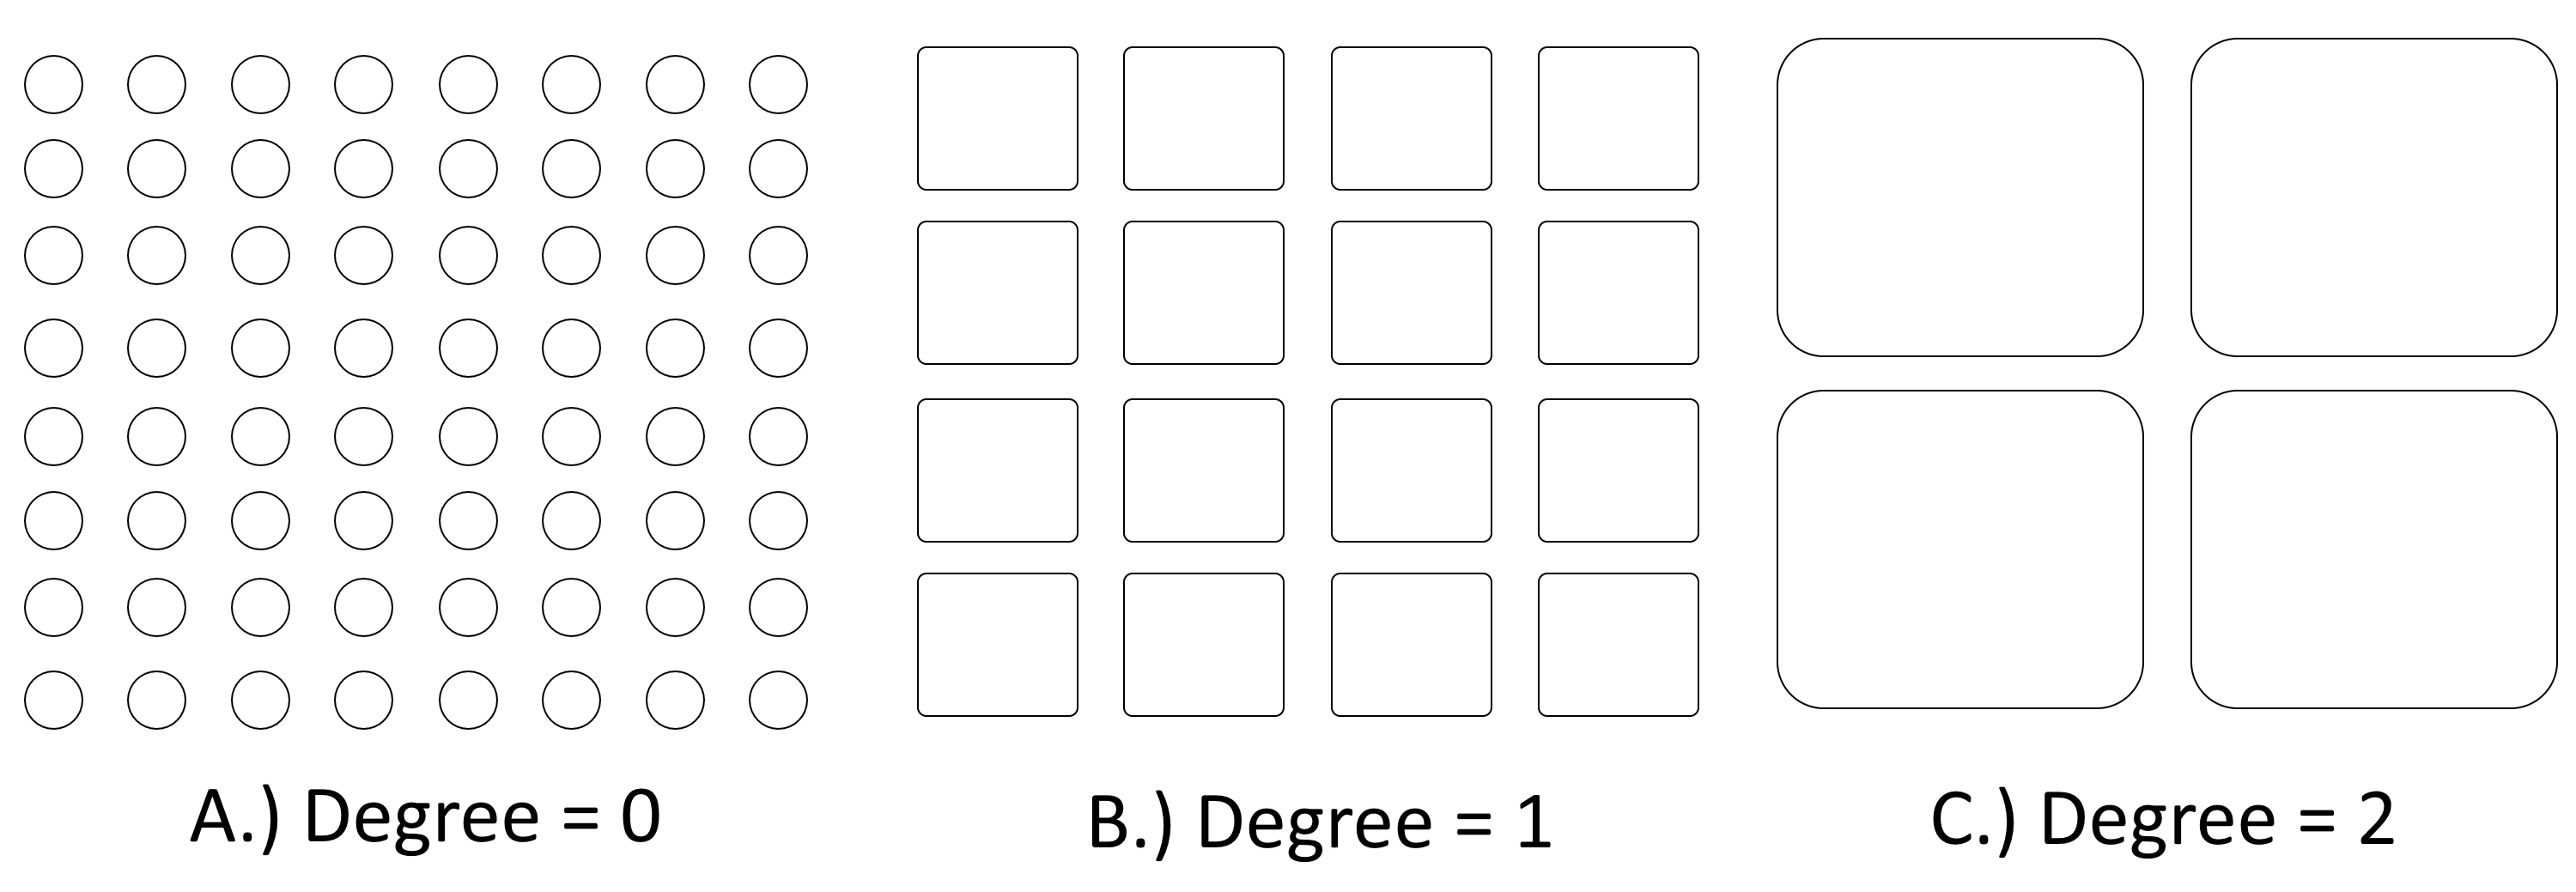
\includegraphics[width=1.0\textwidth]{Figures/ClusterDegree.png}
\caption{\label{fig:CluserDegree} Demonstration of meaning of "Degree" of cluster, a degree of 0 indicated only elements, a degree of 1 represtend cluster of 2x2 elements and a degree of 2 represents clusters of 2x2 clusters of degree 1}
\end{figure} 

It is pertinent to note that all levels of abstraction under and including the maximum degree of abstraction used exist. For example, if a degree of 2 is used, the abstraction layer for a degree of 1 is also calculated. Higher abstractions are always created using the same routine, hence a fractal like recurring pattern is seen if elements from higher degrees are "zoomed" in upon. This is shown in figure \ref{fig:FractalPattern}

\begin{figure}[H]
\centering
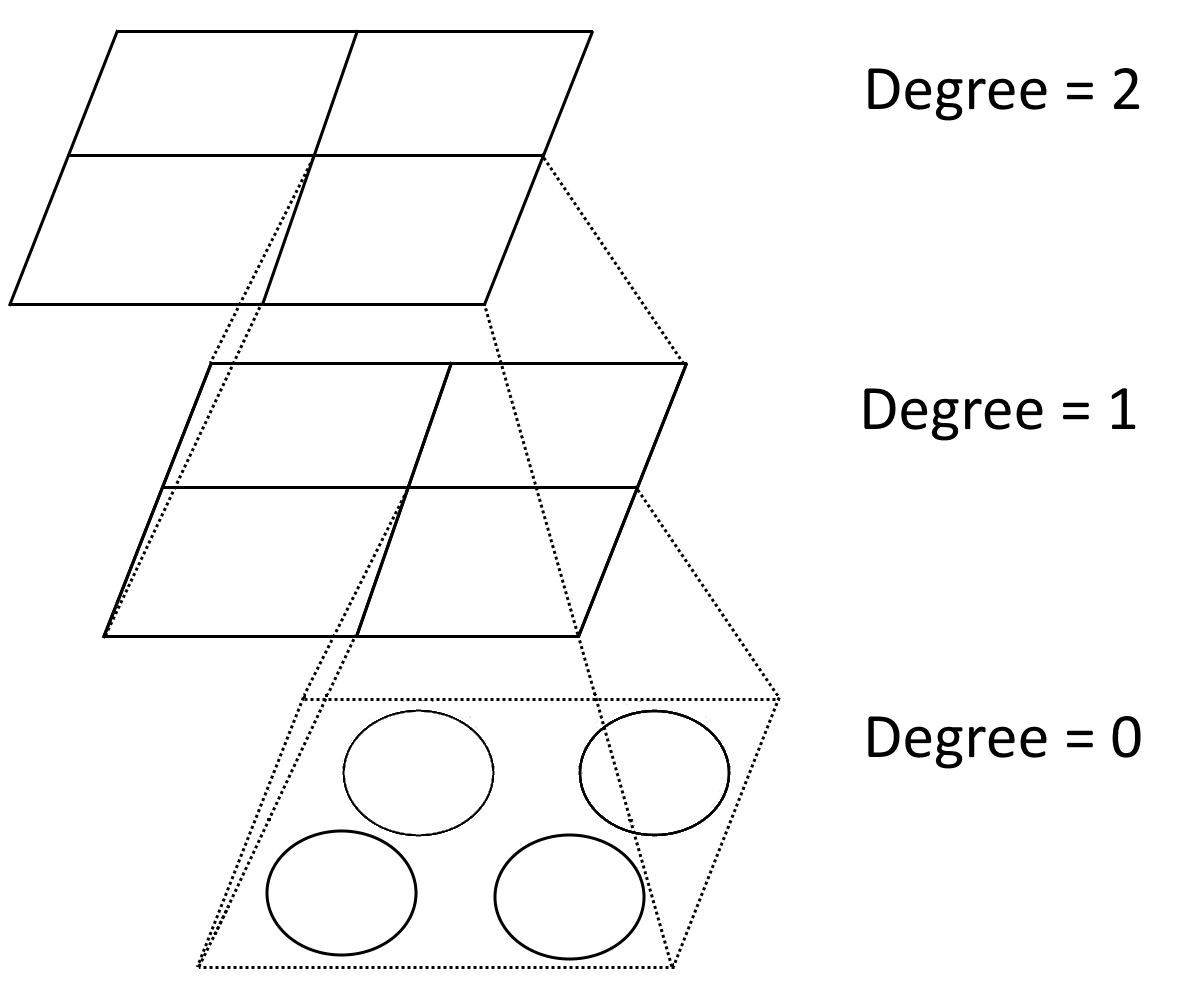
\includegraphics[width=0.6\textwidth]{Figures/FractalPattern.png}
\caption{\label{fig:FractalPattern} Fractal like pattern generated by numerous abstractions applied using the same procedure}
\end{figure} 

Elements are convected by other elements and clusters of every level of abstraction. The maximum degree of abstraction is found by considering the largest degree of abstraction that can be used that results in more than one quadrant being present at the maximum degree. For example, the maximum degree of abstraction that can be used for a $8x8$ grid of elements is 2, this is because $2^2=4$, resulting in 4 quadrants present on the grid, however $2^3=8$ which would result in 1 quadrant which is not allowed.
\\\\
The algorithm convects a single element by considering the maximum degree of abstraction and finding which quadrant the element belongs to. The element is then convected with every quadrant it is not part of and the the quadrant it is part of is "zoomed" in on and the procedure repeated for that level of abstraction. This procedure recurs until all levels of abstraction up to and including 0 have been considered, and so all elements have been taken into account. This gives rise to a pattern of clusters for a given element as demonstrated in figure \ref{fig:AbstractionExample}

\begin{figure}[H]
\centering
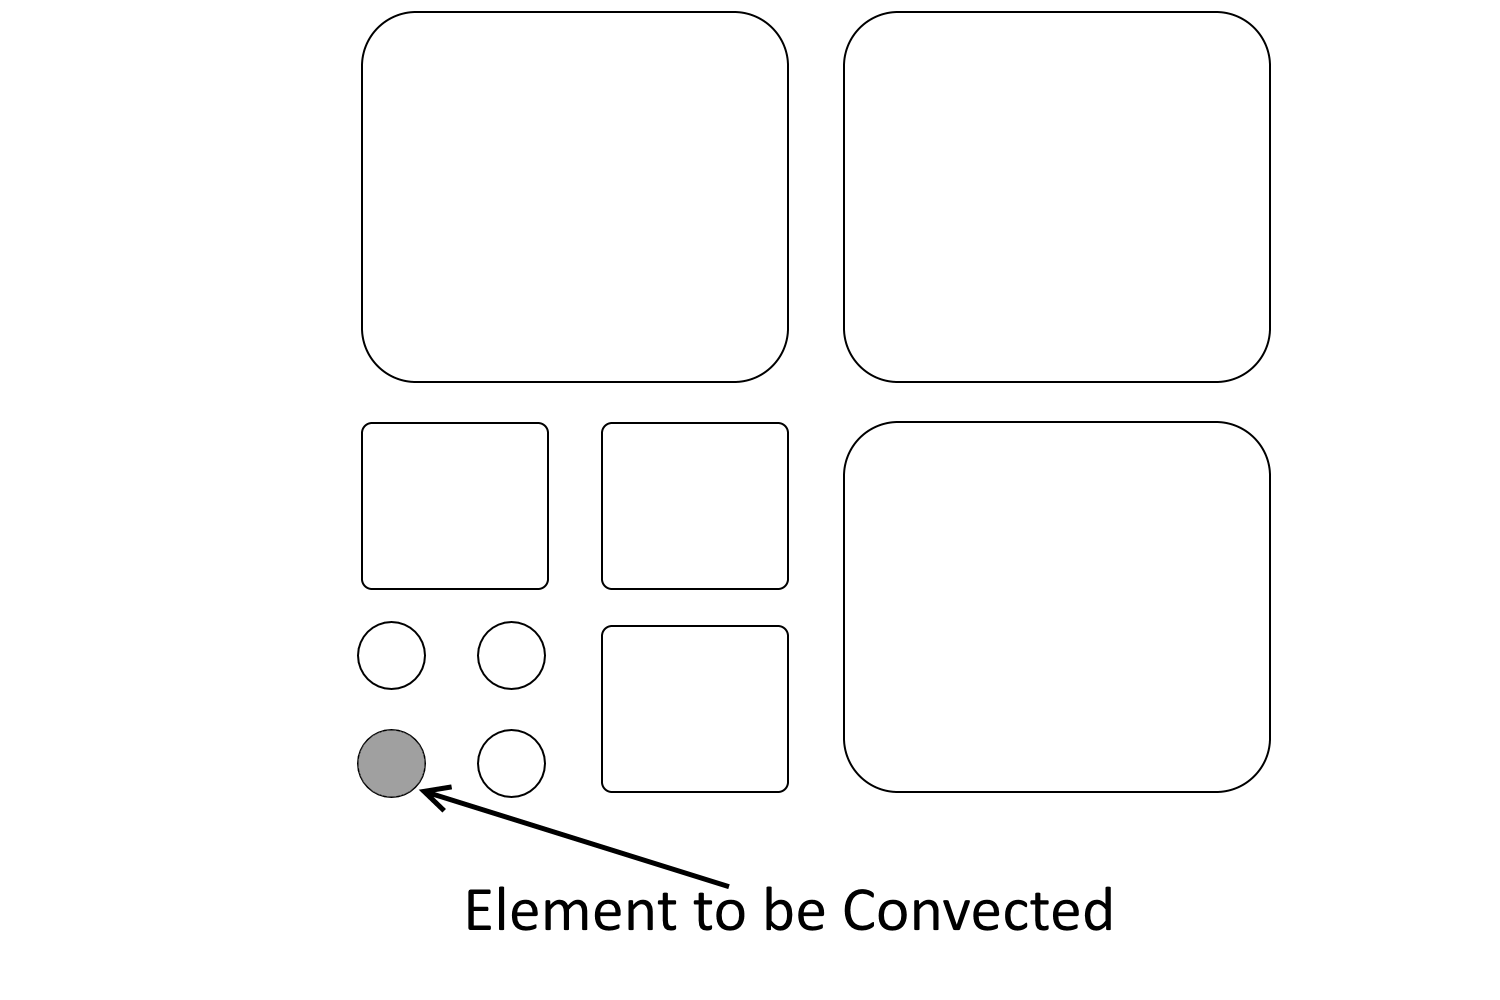
\includegraphics[width=0.7\textwidth]{Figures/DynamicAbstractionExample.png}
\caption{\label{fig:AbstractionExample} Clustering pattern for a given element}
\end{figure} 

Because the implementation of such an algorithm is more complex than the previous schemes the separate steps in the algorithms were segmented into independent functions called from a central function "convectionDispatcher" which dispatches tasks to other functions. This gives rise to a single "black box" function that need only be called in the main loop. This is demonstrated in figure \ref{fig:ProgramStructure}

\begin{figure}[H]
\centering
\includegraphics[width=0.9\textwidth]{Figures/DynamicProgramStructure.png}
\caption{\label{fig:ProgramStructure} Example of "Black Box" nature of the dispatch function}
\end{figure} 

The convection dispatcher function is shown in list \ref{list:ConvectionDispatcher}. Upon inspection it is apparent that the function only calls other functions. The functions findVorticities() and updatePositions() are shared across all schemes and are included in the appendix. The function determineMaximumDegree() determines the maximum abstraction degree that results in more than one quadrant, this function is included in the main loop so that the element count can be varied during the simulation. The function determineCoefficients() uses the maximum abstraction degree to determine the vorticities and positions of all abstraction levels.

\begin{listing}[H]
\begin{minted}[linenos,breaklines]{csharp}
//Function that ties all the parts together
    void convectionDispatcher()
    {

        //Perform Subroutines to find necessary values
        findVorticities();
        determineMaximumDegree()
        determineCoefficients();
        resetAllVelocities();


        //Now we cycle through all elements and run the convection routine
        for (int x = 0; x < xSize; x++)
        {
            for (int y = 0; y < ySize; y++)
            {
                Convect(x, y, maxDegree, 0, xSize, 0, ySize, 0, 0);
            }
        }

        //Now implement the discretizaton scheme
        updatePositions();

    }
\end{minted}
\caption{Entire Convection Dispatcher Function}
\label{list:ConvectionDispatcher}
\end{listing}

On lines 13 to 19 two for loops are present that cycle through every coordinate on the grid, the function Convect() is then called. The Convect() takes the the coordinate of the element and convects it with the appropriate elements and clusters of varying abstraction levels. The entire function is provided in the appendix however its operation is described here in segments.
\\\\

\begin{listing}[H]
\begin{minted}[linenos,breaklines]{csharp}
    //This function finds the appropriate elements and abstracted clusters for the given element 
    void Convect(int xg, int yg, int degree, int xs, int xe, int ys, int ye, int xBias, int yBias)
    {
\end{minted}
\caption{Convect Function Declaration showning all input arguments.}
\label{list:ConvectDecleration}
\end{listing}

The Convect() function takes 9 arguments, these are shown in list \ref{list:ConvectDecleration}. The variables $xg$ and $yg$ specify the elements position on the grid to convect. The variable degree specifies the level of abstraction to be considered, in list \ref{list:ConvectionDispatcher} this is always set to the maximum level of abstraction possible when calling the function. The relevance of this will be discussed later. The variables $xs$, $xe$, $ys$, $ye$ specify the area of the grid of elements to be considered, $xs$ and $xe$ being the x coordinate at the start and end of the grid segment and likewise $ys$ and $ye$ being the start and end of the y coordinates of the grid segment. In reference to list \ref{list:ConvectionDispatcher} again it is seen that these are set so the they specify the entire grid. This is shown in figure \ref{fig:GridNomenclature}. The variables $xBias$ and $yBias$ are discussed later when their relevance becomes apparent.
\begin{figure}[H]
\centering
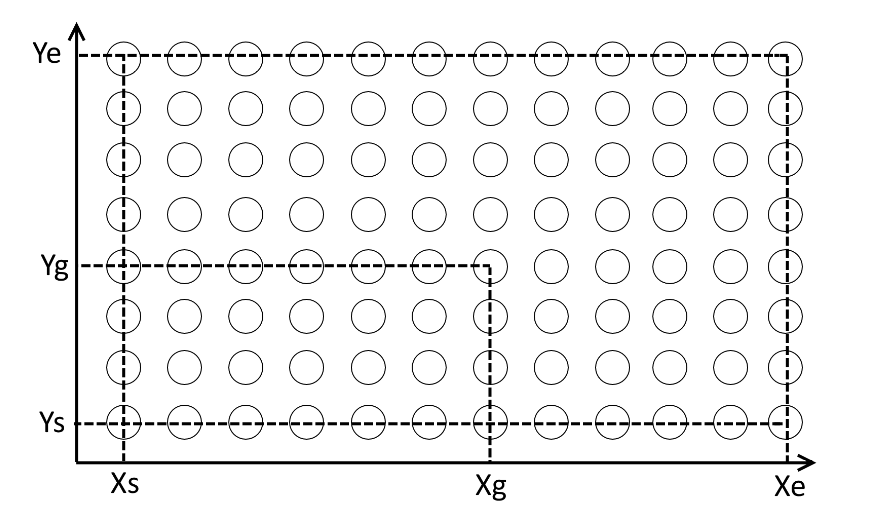
\includegraphics[width=0.6\textwidth]{Figures/AbstractionGridExample.png}
\caption{\label{fig:GridNomenclature} Physical representation of variables used in the Convect() function}
\end{figure} 

The first step for the convective function is to determine the size of the grid it is considering given the specified level of abstraction. This section of the code is shown in list \ref{list:ConvectGridSize}. On line 2 the size of clusters is found in terms of elements, for example a 2x2 cluster of elements has a spacing of 2, though a 2x2 cluster of clusters of degree 1 has a spacing of 4 ($2x2x2$). Once the size of the clusters in terms of elements is known, the size of the grid to be considered is then dived by this spacing to yield the number of segments present, this shown on lines 10 and 11. The evaluation on line 8 handles an anomoly at the boundary (abstraction = 0) where the grid size calcultion returns unity.

\begin{listing}[H]
\begin{minted}[linenos,breaklines]{csharp}
        //determine grid spacing 
        int spacing = (int) Mathf.Pow(clusterSize, degree);


        //first step is to determine the current cluster size
        int xGridSize = 0;
        int yGridSize = 0;
        if (degree != 0)
        {
            xGridSize = (xe - xs + 1) / spacing;
            yGridSize = (ye - ys + 1) / spacing;
        }
        else
        {
            xGridSize = 2;
            yGridSize = 2;
        }
\end{minted}
\caption{Section of the Convect() function that determines the current grid size given the level of abstraction}
\label{list:ConvectGridSize}
\end{listing}

At this point the Convect function has taken a segment of the grid and divided it up into quadrants given the current. Hence the grid representation shown in figure \ref{fig:GridNomenclature} has transformed to figure \ref{fig:GridNomenclature2}.

\begin{figure}[H]
\centering
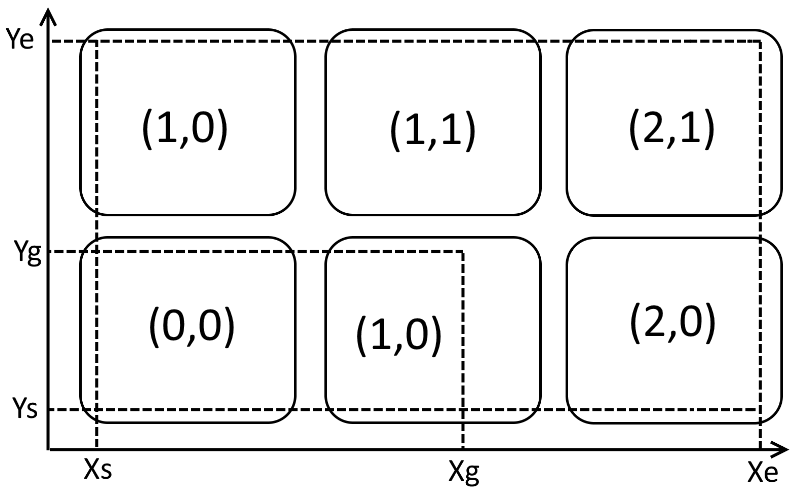
\includegraphics[width=0.6\textwidth]{Figures/AbstractionGridExample2.png}
\caption{\label{fig:GridNomenclature2} Result of the Convect() function splitting the considered grid segment into clusters}
\end{figure} 

The next step of the Convect function is to determine which of these quadrants the element to be convected (at location xg,yg) lies within. This is shown in list \ref{list:ConvectDetermineMyQuadrant}

\begin{listing}[H]
\begin{minted}[linenos,breaklines]{csharp}
//determine current position on the grid
        int xgp = 0;    //start by declaring variables for our position on the "local" grid
        int ygp = 0;    //And againt for the y position
        //for for loops to determine their values
        for (int x = 0; x < xGridSize; x++)
        {
            if ( xg >= (xs + x*spacing) && xg < (xs + (x + 1) * spacing))
            {
                xgp = x;
            }
        }
        //now determine the y coordinate
        for (int y = 0; y < yGridSize; y++)
        {
            if ( yg >= (ys + y * spacing) && yg < (ys + (y + 1) * spacing))
            {
                ygp = y;
            }
        }
\end{minted}
\caption{Section of the Convect() function that determines the grid segment the element to be convected lies within}
\label{list:ConvectDetermineMyQuadrant}
\end{listing}

Now the quadrant the element lies in is known, so the element in question can be convected with the segments it is not in and the segment it is in should be considered at the next lowest abstraction level. This is shown in list \ref{list:ConvectWithSegments}

\begin{listing}[H]
\begin{minted}[linenos,breaklines]{csharp}
//Now cycle through clsuters
        for ( int x = 0; x <  xGridSize; x++)
        {
            for ( int y = 0; y < yGridSize; y++)
            {
                if ( x == xgp && y == ygp)
                {
                    //Check if we're at the base level abstraction
                    if (degree > 0)
                    {
                        Convect(xg, yg, degree - 1, xs + (xgp * spacing), xs + (xgp+1)*spacing, ys + (ygp * spacing), ys + (ygp + 1) * spacing, (xBias + x) * clusterSize, (yBias + y) * clusterSize);
                    }                
                }
                else
                {
                    biotSavart(xg, yg, x + xBias, y + yBias, degree);
                }
            }
        }
\end{minted}
\caption{Section of the Convect() function that either calls the Biot-Savart function or calls itself to consider a lower abstraction level}
\label{list:ConvectWithSegments}
\end{listing}

In list \ref{list:ConvectWithSegments} two for loops (on lines 2 and 4) are used to cycle through the coordinated of all grid segments in figure \ref{fig:GridNomenclature2}. Inside these for loops an evaluation is made to determine whether the current cluster in question contains the element to be convected. If the element is not in that cluster, the function biotSavart() is called and the element is convected with these clusters.
\\\\
If the element is in the cluster however the situation is more complex. First the another evaluation is made, this is shown on line 9. This evaluation determines whether or not the lowest (0) abstraction layer is being considered. If the lowest abstraction level is being considered then nothing needs to be done. However if the element that is to be convected is still in a cluster that cluster then needs to be considered further. This is done by calling the Convect() function from within the Convect() function.
\\\\
The second call to the Convect() function can be seen on  line 11. The arguments passed to this instance of the COnvect() function are different from the initial instance of the function. The values of $xg$ and $yg$ passed to the new function are constant. However the values for $xs$, $xe$, $ys$ and $ye$ now reflect the coordinates of the segment the element was present in. This is demonstrated in figure \ref{fig:GridNomenclature3}.

\begin{figure}[H]
\centering
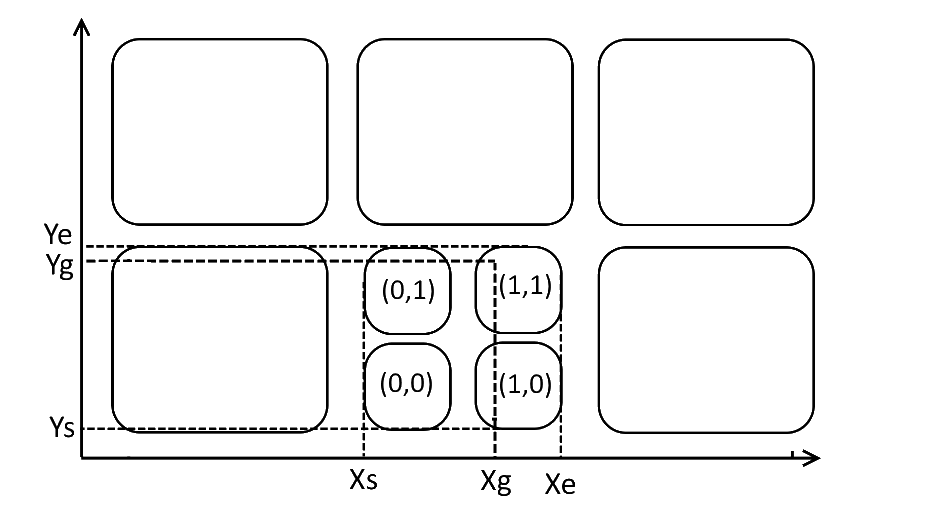
\includegraphics[width=0.7\textwidth]{Figures/AbstractionGridExample3.png}
\caption{\label{fig:GridNomenclature3} Result of the Convect() function splitting the considered grid segment into clusters}
\end{figure} 

Values for $xBias$ and $yBias$ are also passed to the new instance of the Convect() function. These values represents the $x$ and $y$ coordinate of the current cluster multiplied by the cluster spacing. Physically this represents the coordinates of the starting point of the new set of clusters. In the example shown in \ref{fig:GridNomenclature3} this would refer to the coordinate of the cluster $(0,0)$ however on a local global, the the coordinate $(2,0)$ would be given (see figure \ref{fig:GridNomenclature4}). 

\begin{figure}[H]
\centering
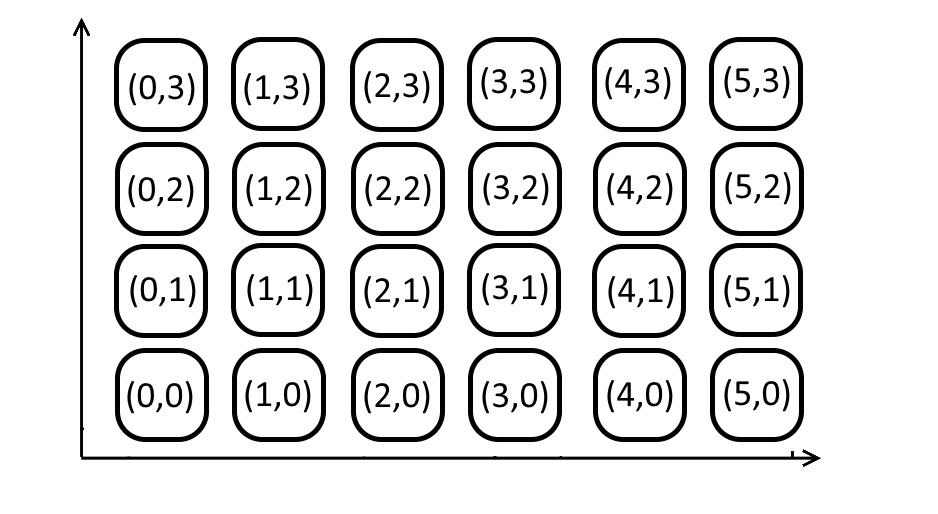
\includegraphics[width=0.7\textwidth]{Figures/AbstractionGridExample4.png}
\caption{\label{fig:GridNomenclature4} Global coordinates of clusters for a single level lower abstraction}
\end{figure} 

These gloabal coordinates are passed to the biotSavart() function when a element is to be convected by a cluster. The biotSavart() function is shown in listing \ref{list:biotSavart}. Its implementation is identical to the Simple Convections scheme with the except of the added dimension to the position and vorticity arrays to account for the degree of clustering.

\begin{listing}[H]
\begin{minted}[linenos,breaklines]{csharp}
//This function implements the biot-savart law maybe
    void biotSavart(int ex, int ey, int cx, int cy, int degree)
    {

        //This calculate the influence
        //First the radius,
        Vector3 radius = elementPosition[ex, ey, 0] - elementPosition[cx, cy, degree];
        //Now the Biot-Savart law itself
        elementVelocity[ex, ey] += (1f / (4f * Mathf.PI)) * (Vector3.Cross(vorT[cx, cy, degree], radius) / (Mathf.Pow(radius.magnitude, 2)));

    }
\end{minted}
\caption{Implementation of the Biot-Savart law for the dynamic clustering scheme}
\label{list:biotSavart}
\end{listing}